% \chapter{重建算法分类}
表面重建重建是经典的计算机图形学任务之一,传统手段分为\textit{显式重建}、\textit{隐式重建}两种;而近几年又有很多\textit{深度学习重建}的算法喷涌而出。\\

\textit{显式重建}会通过\textit{Delaunay三角剖分}或\textit{Voronoi图}直接划分原始点云数据,构造其几何结构;\textit{隐式重建}则是学习一个隐函数,来明确哪些是模型内点,哪些是外点。\\

因为遮挡及仪器精度问题,原始点云存在很多噪音,比如离群点、遮挡导致的空洞等,\textit{显式重建}会把噪音建模其中,而\textit{隐式重建},通过隐函数处理此类问题,对噪音的处理及容忍度更高,效果也更好一些。\\

\section{指示函数}
常通过定义一个$3$值指示函数来区分模型内外的点,比如点在模型外,则函数值为$-1$;在内为$1$;在表面上,则为$0$;后续建模的主要工作便是学习出这个指示函数,从而确定模型表面。\\

但本文使用的是一个$2$值指示函数$\mathbf{\chi}_M$:点在模型外为$0$,在模型内(包括表面)为$1$。
\begin{figure}[H]
		\begin{center}
			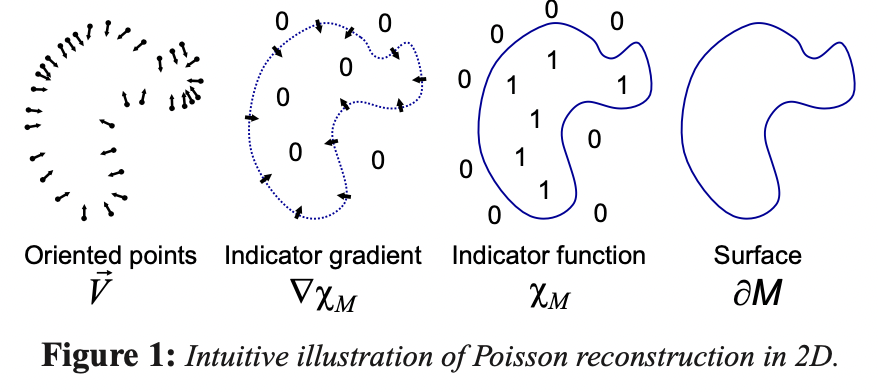
\includegraphics[scale=0.8]{images/p1.png}
		\end{center}
\end{figure}

指示函数$\mathbf{\chi}_M$是一个分段常值函数,在模型内外,梯度均为$0$,但在表面附近梯度为无穷大,并且梯度方向是表面点的\textit{内法向量}(多元函数,某点梯度即为该点法向)。\\

这表明,指示函数与表面点之间存在对应关系。但表面点梯度不存在,导致指示函数无法被求解,通常通过与某个光滑函数$\tilde{F}$作卷积,构造一个新的指示函数$\tilde{\chi}$,新指示函数与表面点之间的关系,由如下引理描述:

\begin{equation}
	\nabla \tilde{\chi}(q_0) = \nabla(\chi_M * \tilde{F})(q_0) = \int_{\partial{M}}\tilde{F}_p(q_0)\overrightarrow{N}_{\partial{M}}(p)d_p \label{lemma_1}
\end{equation}

$\overrightarrow{N}_{\partial{M}}(p)$为$p$点的\textit{内法向量}。\\

引理表明,指示函数与卷积核的梯度,等于卷积核与法向量在模型表面的积分,这是$\tilde{\chi}$与表面点法向之间的对应关系,原文中称为积分关系。\\

在证明这个结论之前,先复习一下\textbf{格林公式}/\textbf{散度定理}:\\


$M$为模型,$S$为模型表面(等同于文中的$\partial M$),$\mathbf{n}$为$S$的\textit{外法向量},$\mathbf{F}$为定义在$S$上的向量场,则\textbf{格林公式}/\textbf{散度定理}结论为,
$$
\iint_{S}\mathbf{F}\cdot\mathbf{n} \text{ } d \mathbf{S} = \iiint_M \mathop{div} \mathbf{F} \text{ }  dV 
$$

其中,$P(x,y,z), Q(x,y,z), R(x,y,z)$为向量场$\mathbf{F}$对应的三个坐标函数,
$$
div \mathbf{F} = \frac{\partial P}{\partial x} + \frac{\partial Q}{\partial y} + \frac{\partial R}{\partial z}
$$
为$\mathbf{F}$的散度。\\

\textbf{格林公式}/\textbf{散度定理}表明,向量场与法向的\textbf{面积分}等价于向量场散度的\textbf{体积分}。\\

只要验证(\ref{lemma_1})式左侧$\tilde{\chi}$的梯度等于(\ref{lemma_1})式右侧,引理即可证明,

\begin{align}
	\frac{\partial}{\partial x}\bigg |_{q_0} (\chi_M * \tilde{F}) &= \frac{\partial}{\partial x}\bigg |_{q_0} \int_M \tilde{F}(q-p) \mathop{d}p \label{proof_1}\\
	&= \int_M \left(-\frac{\partial}{\partial x}\tilde{F}(q_0 - p)\right)\mathop{d}p \label{proof_2}\\
	&= -\int_M \nabla \cdot \left(\tilde{F}(q_0 - p),0,0\right)\label{proof_3}\\
	&= \int_{\partial M}
		\left <
			\left(
				\tilde{F}_p(q_0),0,0
			\right)
			,
			\overrightarrow{N}_{\partial M}(p)
		\right>\mathop{d}p \label{proof_4}
\end{align}

上式只是对$x$进行求导,对$y,z$求导也可得出类似结论,从而引理得到证明。\\

(\ref{proof_1})是指示函数与卷积函数的卷积结果;(\ref{proof_2})是将$\tilde{F}$对$q$的求导转换为对$p$的导数;(\ref{proof_3})是将积分写为散度的形式;(\ref{proof_4})是根据\textbf{格林公式}将体积分转变为面积分。

\section{梯度场的求解}

\subsection*{积分中值定理}
	对函数$f(\mathbf{x})$在区域$\mathbf{D}$上的积分,存在某个$\mathbf{x}_0$,使得下式成立,
	$$
		\int_D f(\mathbf{x}) \mathop{d}\mathbf{x} = |\mathbf{D}|f(\mathbf{x}_0)
	$$

	$|\mathbf{D}|$是积分区域大小,若$f$为二元函数,$|\mathbf{D}|$为面积;为三元函数,则为体积。

\subsection*{梯度场近似计算}
将$\partial M$划分为一些列互不相交的集合$\mathcal{P}_s$,在每个$\mathcal{P}_s$上,对积分进行求和,

\begin{align}
	\nabla (\chi_M * \tilde{F})(q) &= \sum_{s \in S}\int_{\mathcal{P}_s}\tilde{F}_p(q)\overrightarrow{N}_{\partial M}(p)\mathop{d}p\\
	&\approx \sum_{s \in S}|\mathcal{P}_s|\tilde{F}_{s.p}s.\overrightarrow{N} \equiv \overrightarrow{V}(q) \label{vector_field}
\end{align}

第二步近似计算是用$p$点的值,代替了\textbf{积分中值定理}中某个确定点$p_0$的值。\\

$|\mathcal{P}_s|$为分割表面积,如果采样是均匀的,可以认为是一个常数,在计算中可以忽略;如果采样是非均匀的,则需自适应计算其大小,后边专门讨论。\\

样本点的法向是确定的,只要卷积核确定,向量场$\overrightarrow{V}(q)$就是可计算的。至此(\ref{lemma_1})式右侧已完全确定,要求左侧指示函数$\tilde{\chi}$,需求解下面变分方程,

$$
\nabla \tilde{\chi} = \overrightarrow{V}
$$

$\nabla \tilde{\chi}$为$\tilde{\chi}$的梯度场,梯度场的特点是旋度(curl)为0,而$\overrightarrow{V}$为一般的向量场,一般来说旋度不为0,因此上述变分方程可能无解。

\subsection*{泊松方程}

对此可放宽条件,用最小二乘的思路,求与$\overrightarrow{V}$距离最小的解,距离可用下面的$L_2$范数定义,

$$
	\mathop{L}(q) = \int \left(\nabla\tilde{\chi} - \overrightarrow{V}\right)^2 \mathop{d}p
$$

求解最小值时的变分,可得$\mathop{L}$最小时需满足,
$$
	\nabla(\nabla \tilde{\chi}) = \nabla\overrightarrow{V} \Rightarrow \Delta \tilde{\chi} = \nabla\overrightarrow{V}
$$

这个方程称为\textit{泊松方程},是一个非齐次二阶偏微分方程。将向量场的求解转变为泊松方程,在物理学中比较常见,所以原文中并未介绍泊松方程的过程。

\section{泊松方程求解}

	泊松方程的直接求解依赖初值条件,这里无法准确建立模型的初值条件,所以无法获得解析解,转而寻求数值解。\\

	为了求得数值解,需要将指示函数$\tilde{\chi}$和向量场$\overrightarrow{V}$在一组函数基下展开,只要确定在这组函数基下的系数便可准确刻画指示函数和向量场,如此泊松方程求解可简化为线性方程求解问题。\\

	那应该在什么函数基下展开呢?

	\subsection{函数基}
		通常可以把一个函数通过泰勒级数或傅里叶变换展开,而在小波变换中,常用小波基展开一个信号,傅里叶基与小波基是正交基,而泰勒基是幂函数,并非正交基。\\

		除了正交性的差异,傅里叶变换与泰勒级数并非\textbf{紧支撑},也就是其定义域是整个函数定义域,而小波基是分段函数,每个基是\textbf{紧支撑}的。\\

		紧支撑使得函数基仅在支撑集上有定义,非支撑集上为0,从而形成\textbf{稀疏性},具体计算时节省计算资源。

	\subsection{函数基选择标准}
		小波基是通过平移、缩放一个小波母函数而得到,因此小波可以做到多分辨分析,而傅里叶变换则做不到。实际上正是因为傅里叶变换做不到多分辨分析,才有了小波变换。\\

		我们希望选择的函数基是紧支撑、稀疏的,在接近模型表面的地方分辨率更高一些,其他地方分辨率稀低一些,这样能更好的的为表面细节建模,同时又节省计算资源,因此文中选择了与小波基类似的函数基。

	\subsection{函数空间}
		设母函数为$F$,通过八叉树把3D空间离散化,使得每个样本点都落在八叉树的叶节点中,此时得到的树的深度为$D$,称为最小生成树。\\

		对每一个叶节点$o$,将母函数平移、缩放得到定义在$o$中心上的函数基$F_o$,
		\begin{align}
			F_o(q) \equiv F\left(\frac{q-o.c}{o.w}\right)\frac{1}{o.w^3} \label{wavelet_func}
		\end{align}

		$o.c$,$o.w$分别是节点$o$的中心和宽度。母函数积分为1,可验证$F_o$的积分也为1;因为树的深度为$D$,所以$o.w = 2^{-D}$\\

		那母函数$F$怎么选择呢?文中选择了方差为$o.w$的单位高斯函数,但高斯函数并不是紧支撑函数,不符合前面讨论的稀疏化的要求,所以通过\textbf{门函数}的$n$次卷积来代替高斯函数。

		\subsubsection*{门函数}
			$$
				B(t) = \left\lbrace 
					\begin{aligned}
						1 \qquad &|t| < 0.5 \\
						0 \qquad &\text{others}
					\end{aligned}
				\right.
			$$

			门函数满足概率密度定义,是一个紧支撑的均匀分布,$\mathbb{E}[B] = 0, \mathop{var}(B) = 1/12$\\

			$n$次卷积为,
			$$
				F(x,y,z) = \left(B(x)B(y)B(z)\right)^{*n}
			$$

		\subsubsection*{随机变量和分布逼近高斯函数}

			为什么门函数的$n$次卷积可以代替高斯函数?在概率论中有下面两个结论,
			\begin{itemize}
				\item $n$个独立同分布随机变量$X_i$和的分布等于$n$个分布的卷积,即:
				$$
					p\left(\sum_{i=1}^nX_i\right) = p(X_1) * p(X_2) * \cdots * p(X_n)
				$$
				\item 根据中心极限定理,
				$$
					\frac{\sum_{i=1}^nX_i - n\mu}{\sqrt{n}\sigma} \sim \mathcal{N}(0, 1)
				$$

				令$Y_n = \frac{\sum_{i=1}^nX_i - n\mu}{\sqrt{n}\sigma}$,当$n->\infty$时,服从标准正态分布,则

				$$
					\sum_{i=1}^nX_i  = \sqrt{n}\sigma Y_n + n\mu
				$$

				近似服从$\mathcal{N}(n\mu, n\sigma^2)$的正态分布,考虑分布为门函数的场景,

				$$
					\sum_{i=1}^nX_i \sim \mathcal{N}(0, n/12)
				$$

				$\sum_{i=1}^nX_i$近似服从$\mathcal{N}(0, n/12)$的正态分布,$n$越大越逼近正态分布,但方差也会越大,所以在本文中作者选择$n=3$
			\end{itemize}

			根据上面讨论,任何一个概率分布的$n$次卷积都可以逼近高斯函数,包括门函数。

		\subsubsection*{门函数$n$次卷积}
			门函数的$n$次卷积是一个分段连续函数,$n$越大分的段数越多,下面是$n=3$的表达式\footnote{\url{https://zhuanlan.zhihu.com/p/627947671}},

			$$
				f_3 = \left\lbrace 
					\begin{aligned}
						&1,  &\quad |t| \leq \frac{1}{8}\\
						&1 - 4\left(\frac{1}{8} - |t|\right)^2, & \quad\frac{1}{8} < |t| < \frac{3}{8}\\
						&2\left(\frac{3}{4} - |t|\right), & \quad \frac{3}{8} < |t| < \frac{5}{8}\\
						&4\left(\frac{7}{8} - |t|\right)^2, & \quad \frac{5}{8} < |t| < \frac{7}{8}\\
						&0, & \quad \text{otherwise}
					\end{aligned}
					\right .
			$$

			实际是一个一次函数和二次函数组合的分段函数,下面是函数图像,虽然只是$n=3$,但已经与正态分布有点相像。

			\begin{figure}[H]
				\begin{center}
					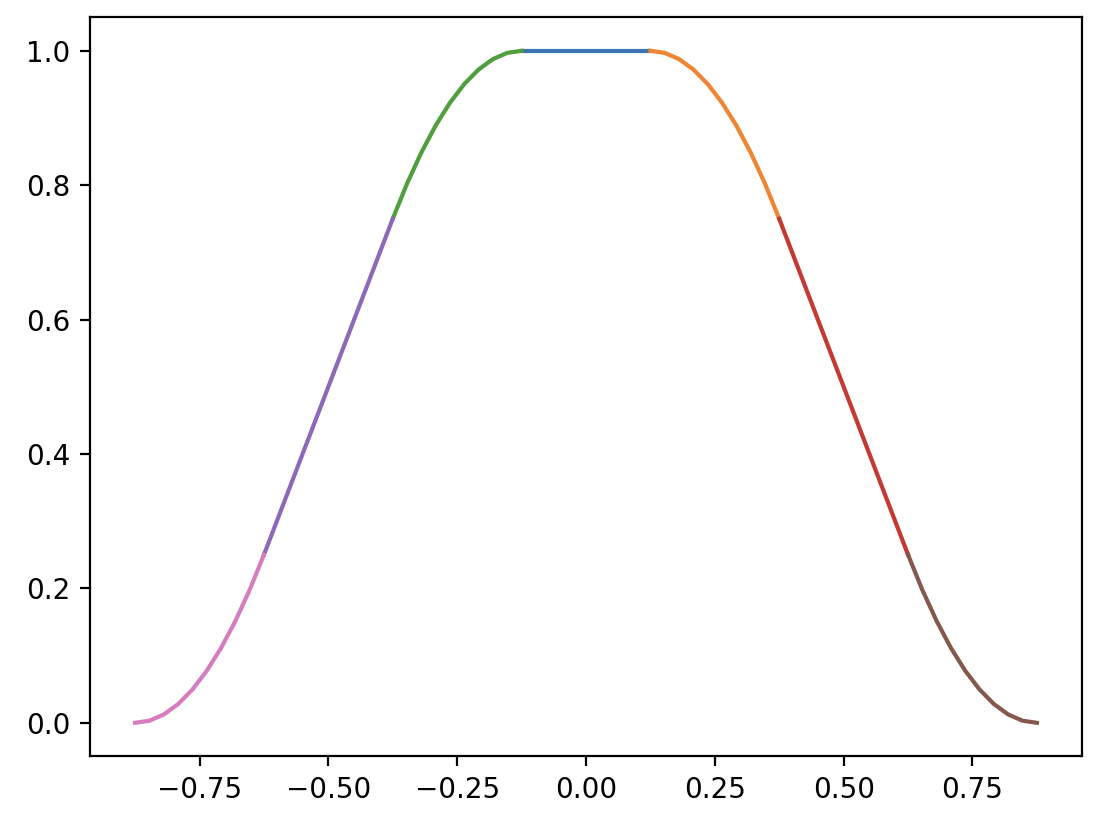
\includegraphics[scale=0.8]{images/p_2.png}
					\title{门函数的三次卷积}
				\end{center}
			\end{figure}

	\subsection{指示函数分解}
		根据前面选定的函数基,就可以按(\ref{wavelet_func})的方式将其进行平移、缩放,定义到八叉树的叶子的中心点上,对指示函数$\tilde{\chi}$,可以用该函数基进行分解,

		$$
			\tilde{\chi}(q) = \sum_{o \in S} \alpha_{o} F_o(q)
		$$

		后续任务是求解出系数${\alpha_{o}}$,但这组函数基并非是正交基,无法像傅里叶变换和小波变换一样,通过积分简单计算其分量。

	\subsection{向量场的分解}
		在向量场(\ref{vector_field})中的卷积函数与前面定义的函数基有什么关系?\\

		基函数通过平移缩放到八叉树叶节点的中心,而向量场的样本点不一定在叶节点的中心上,因此可能被周边多个叶节点上的基函数所覆盖,所以样本点对应的值由邻居加权更为合理,这实际是高斯混合模型的思路,文中通过三线性插值确定分量系数。\\

		文中取了周边最近的8个邻居作插值计算,向量场可分解为:

		\begin{align}
			\overrightarrow{V}(q) = \sum_{s \in S}\sum_{o \in {Ngbr}_D(s)} \alpha_{o,s}F_o(q)s.\overrightarrow{N}
		\end{align}

		系数${\alpha_{o,s}}$在插值过程中确定。\\

		要注意的是\textit{向量场}不同于\textit{向量空间},向量空间的基是一组线性无关的向量;\textit{向量场}是定义在流形之上的向量函数,需用函数基进行分解。\\

		另外,\textit{向量空间}的曲率为0,而\textit{向量场}的曲率一般不为0。


	\subsection{求解Poisson方程}
		我们将指示函数$\tilde{\chi}$与向量场$\overrightarrow{V}$用基函数展开,但$\Delta{\tilde{\chi}}$与$\nabla \overrightarrow{V}$是另外两个不同的函数,这两个函数是否需要在基函数上展开呢?\\

		如果继续展开会导致待定系数过多,没有足够的条件求解,文中用一个折中而又巧妙的处理:只要这两个函数在基函数${F_o}$上的投影足够接近就行,

		$$
		\sum_{o \in \mathcal{O}}\left\Vert \Delta{\tilde{\chi}} - \nabla\cdot \overrightarrow{V}, F_o \right\Vert^2 
		= 
		\sum_{o \in \mathcal{O}}\left\Vert \big<\Delta{\tilde{\chi}}, F_o\big> 
			- 
			\big<\nabla\cdot \overrightarrow{V}, F_o\big> \right\Vert^2
		$$

		这种巧妙处理本质是规避了去刻画两个函数绝对“接近”,而只是追求部分接近(投影),这种处理是否是well-defined呢?\\

		衡量两个函数是否接近,依赖“接近”的度量方式,基函数空间$\{F_o\}$没有上明确定义度量(metric)方式,导致${F_o}$并非是一个度量空间,此处实际就是补充投影内积作为度量方式。\\

		通过内积定义的距离,不但是well-defined,很多时候还是完备的;这个定义虽然合理,但不一定最优,也可以尝试其他度量定义方式。\\

		如此,Poisson问题可转变为一个最小二乘问题,

		$$
			\min_{x\in \mathbb{R}^{|\mathcal{O}|}} \left\Vert Lx - \nu\right\Vert
		$$

		其中,$L$是一个$|\mathcal{O}| \times |\mathcal{O}|$对称正定矩阵,其中每一项内容为,

		$$
			L_{o,o^{\prime}} = \left< \frac{\partial^2 F_o}{\partial x^2}, F_{o^{\prime}}\right>
				+ \left< \frac{\partial^2 F_o}{\partial y^2}, F_{o^{\prime}}\right>
				+ \left< \frac{\partial^2 F_o}{\partial z^2}, F_{o^{\prime}}\right>
		$$

		函数基是紧支撑的,所以通过Gauss-Seidel方法能较快求解这个稀疏的最优化问题。

\section{等值面抽取}
	有了指示函数$\tilde{\chi}$就可以回答某个点在模型内外,	通过\textit{Marching Cubes}\footnote{\url{https://www.cs.carleton.edu/cs_comps/0405/shape/marching_cubes.html}}的方法,刻画出模型表面结构。\\

	为了使用\textit{Marching Cubes},首先需要构建一个等值(isovalue),以此计算\textit{Marching Cubes}每个立方体8个顶点的等值,如果8个顶点的等值不相同,则等值面会穿过这个立方体,从而插值的方式构造立方体的切面来拟合出\textit{等值面}。\\

	一般用样本的均值来构建等值,文中也不例外,\textit{等值面}定义如下,

	$$
		\partial M \equiv \left\lbrace q \in \mathbb{R}^3 \mid \tilde{\chi}(q) = \gamma\right\rbrace
	$$

	$\gamma$为等值,

	$$
		\gamma = \frac{1}{|S|} \sum_{s \in S}\tilde{\chi}(s.p)
	$$

	那$\tilde{\chi}(s.p)$具体是什么值?这个均值定义是否会使得偏离均值的样本点被划分到表面之外?计算一下,

	$$
		\tilde{\chi}(q) = \chi(q) * \tilde{F}(q) = \int \tilde{F}(q-p)\mathop{d}p = 1
	$$

	最后一步,基函数平移缩放但保持积分不变。根据指示函数定义,这个等值实际就是模型表面的值,等值面就是模型表面。\\

	那为啥不直接把等值定义为1呢?在算法计算过程中存在误差,使得计算值偏离理想值1,用实际计算结果会更加鲁棒。

\section{非均匀采样}
	如果样本采样并非均匀分布,(\ref{vector_field})式中梯度场计算时,$|\mathcal{P}_s|$就不能再认为是常数,具体值需由该点的密度决定。\\

	评估样本点的分布,通常用\textit{非参数估计},或者更具体的\textit{核概率密度估计},本文也是这个思路,给出下面的密度估计函数,

	对给定的深度$\hat{D} < D$,
	$$
		W_{\hat{D}}(q) \equiv \sum_{s \in S} \sum_{o \in {Ngbr}_{\hat{D}}(s)} \alpha_{o,s}F_o(q)
	$$

	还是通过卷积函数来模拟密度估计,这个方式实际与原始的\textit{核概率密度估计}差异较大,但一定程度上也可能刻画样本疏密程度。\\

	基于新的密度评估函数,重写(\ref{vector_field}),
	\begin{equation}
		\overrightarrow{V}(q) = \sum_{s\in S}\frac{1}{W_{\hat{D}}(s.p)} \sum_{o \in {Ngbr}_D(s)} \alpha_{o,s}F_o(q) \label{vector_field_v2}
	\end{equation}

	除了考虑样本局部密度,还需考虑卷积核的宽度与密度匹配,密度大的地方用小尺寸卷积核,提升细节分辨率;密度小的地方用大尺寸卷积核,更好的平滑噪音。\\

	具体来说,密度越大的地方用更大的深度(但不超过深度为$D$);密度小的地方,用更小的深度;卷积核尺寸的变化体现在通过不同深度的邻居节点进行插值。\\

	(\ref{vector_field_v2})继续修改为,

	\begin{equation}
		\overrightarrow{V}(q) = \sum_{s\in S}\frac{1}{W_{\hat{D}}(s.p)} \sum_{o \in {Ngbr}_{Depth(s.p)}(s)} \alpha_{o,s}F_o(q) \label{vector_field_v3}
	\end{equation}

	其中,

	$$
		{Depth}(s.p) \equiv \min\left(D, D + \log_4\left(W_{\hat{D}(s.p)}/W\right)\right)
	$$

	$W$是平均采样密度。${Depth}(s.p)$会根据当前点的密度与平均密度自适应深度变化。\\

	同样,等值面也需重写,

	$$
		\partial M \equiv \left\lbrace q \in \mathbb{R}^3 \mid \tilde{\chi}(q) = \gamma \right\rbrace
		\qquad \text{with} \quad  \gamma = 
				\frac{
					\sum \frac{1}{ W_{\hat{D}}(s.p)} \tilde{\chi}(s.p)
				}
				{
					\sum \frac{1}{ W_{\hat{D}}(s.p)}
				}
	$$

\section{总结一下}
	在传统方法中,泊松重建的效果是最好的,主要原因是泊松重建算法从整体优化建模,并且隐函数的建模方式抗噪能力较强。\\

	具体实现上通过类似小波函数的函数基作指示函数和向量场的分解,相比傅里叶基,小波基有多分辨分析的优势。但根据文中实验结果看起来基于傅里叶基的效果也不差。